% TODO: ARRIVATO A PAGINA 12
%TODO: skippato da pagine 61, DA FARE
% WARN: PARTO DA PAGINE 69

\chapter{Telecomunicacion network basics}
\section{The OSI and Internet models}

L'architettura \textbf{Open System Interconnetion(OSI)} punta a collegare sistemi
eterogenei fra di loro, la sua specifica è la \textbf{ISO 7498} ed è un modello
costituito di 7 \textit{strati}.

\begin{figure}[!ht]
	\centering
	% TODO: ingrandire immagine a 0.4
	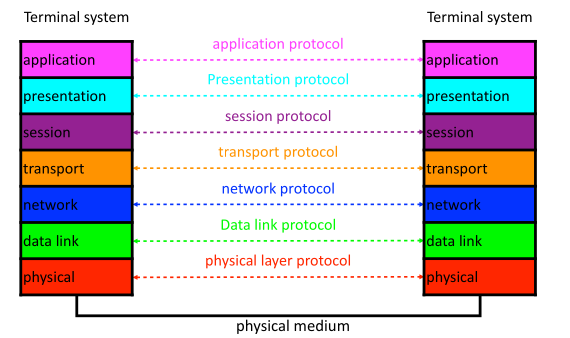
\includegraphics[width=0.4\columnwidth]{./images/osi.png}
	\caption{Architettura OSI}
	\label{fig:osi}
\end{figure}

\subsection{Application Layer}
Livello del modello OSI dove le applicazioni accedono ai servizi di rete, permette ad esempio
di trasferire un file, connettersi a database, uso di mail, ecc.

\subsection{Presentation Layer}
Livello del modello OSI adibito alla trasmissione di dati, traduce differenti formati di dati 
presenti nell'Application Layer in uno standard per gli strati inferiori.

Fornisce servizi per la trasmissione sicura ed efficiente dei dati come:
\begin{itemize}
  \item data encryption
  \item data compression
  \item altre
\end{itemize}

\subsection{Session Layer}

Livello del modello OSI che permette due computer diversi di \textbf{creare}, \textbf{usare}
e \textbf{finire} una sessione, utile per trasmissione di dati e accesso in remoto.

Introduce:
\begin{itemize}
  \item \textbf{Controllo di dialogo}: per regolare la trasmissione e la durata delle stesse
  \item \textbf{Gestione dei token e sincronizzazione}
\end{itemize}

\subsection{Transport Layer}
Livello del modello OSI adibito alla gestione dei pacchetti da trasmettere:
\begin{itemize}
  \item Divide pacchetti grandi in più piccoli
  \item Riordina i pacchetti nell'ordine correto all'arrivo
\end{itemize}

Gestisce inoltre il riconoscimento degli errori e il loro recupero:
\begin{itemize}
  \item Ricezzione di pacchetti di confermo dell'arrivo (ACK)
  \item Reinvia pacchetti persi
\end{itemize}


\subsection{Network Layer}
Livello del modello OSI adibito alla gestione dell'instradamento dei dati attraverso le sottoreti:
% TODO: ARRIVATO A PAGINA 12














\section{Communication models}
\section{Delimitation}
\section{Sequence control}
\section{Error management}

Il controllo dell'errore ha 3 possibili soluzioni:
\begin{itemize}
	\item \textbf{Error detection}: rilevazione dell'errore
	\item \textbf{Error correction}: correzione dell'errore
	\item \textbf{Error recovery}: recupero dell'errore
\end{itemize}

\subsection{Complement sum}

\begin{figure}[!ht]
	\centering
	% TODO: ingrandire immagine a 0.4
	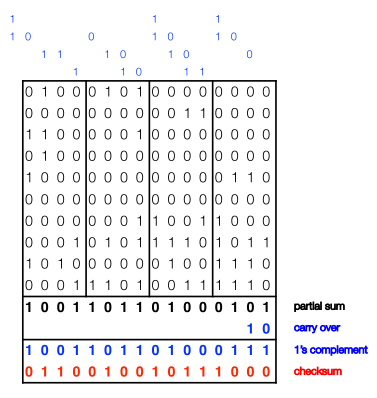
\includegraphics[width=0.4\columnwidth]{./images/complement_sum.png}
	\caption{Complement sum}
	\label{fig:complement_sum}
\end{figure}

Quando si riceve il pacchetto, si calcola il \textbf{checksum} dei dati ricevuti(come in \autoref{fig:complement_sum})
e lo si confronta al checksum allegato al pacchetto ricevuto,
nel caso di checksum differente si deve ritrasmettere il pacchetto.

\subsubsection{Other codes}

\textbf{Polynomial codes} conosciuti anche come \textbf{Cyclic Redundancy Check(CRC)},
usano moltiplicazioni tra polinomi per effettuare il checksum.

\subsection{Error correction}
Con la \textbf{block parity check} si possono recuperare errori ma solo se presente un errore di 1 bit.

Vengono quindi introdotte tecniche \textbf{Forward Error Correction(FED)}(\href{https://en.wikipedia.org/wiki/Viterbi_algorithm}{ad esempio Algoritmo di Viterbi})
che permettono di capire la presenza di un errore mediante algoritmi di ricostruzione.

Con FED si ricorre a ridondanza per eliminare errori(pochi in numero), non sono necessari messaggi
di corretta ricezione, che torna molto utile nel caso di comunicazione unidirezionale.


\begin{figure}[!ht]
	\centering
	% TODO: ingrandire immagine a 0.4
	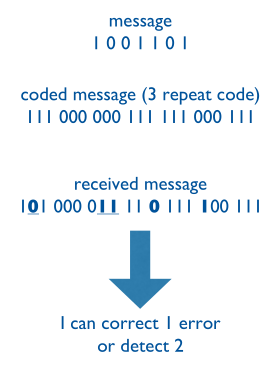
\includegraphics[width=0.4\columnwidth]{./images/repetition_code.png}
	\caption{Repetition code}
	\label{fig_repetition_code}
\end{figure}

\section{Error recovery}

Quando si parla di comunicazione in reti di comunicazioni, si ricade nel richiedere automaticamente
un pacchetto che non risulta corretto al ricevitori,
esistono approcci automatici come \textbf{Automatic Repeat Request, ARQ}.

Esistono inoltre differenti meccanismi di ritrasmissione che come punto focale hanno:
\begin{itemize}
	\item Error detection
	\item Acknowledgements
	\item timers
	\item IU identifiers
\end{itemize}


Le procedure ARQ cambiano in base alla dimensione delle finestra:
\begin{itemize}
	\item \textbf{Stop and wait}: finestra di dimensione 1, si attende l'ack prima di inviare il pacchetto successivo
	\item \textbf{Sliding window, go-back-N}: finestra di dimensione N, si inviano N pacchetti prima di attendere l'ack(non ha un selettore per il resending e invia tutto il blocco)
	\item \textbf{Sliding window, selective repeat}: finestra di dimensione N, si inviano N pacchetti prima di attendere l'ack(ha un selettore per il resending e invia solo il pacchetto corrotto)
\end{itemize}


\subsubsection{Stop and Wait}

Il pacchetto \textbf{ACK(acknowledgement)} solitamente è molto corto per evitare
correzzioni nel pacchetto che conferma la corretta ricezione.

È necessario stabilire un tempo limite entro il quale si da per scontato
la \textit{scomparsa} del pacchetto, solitamente si basa sul \textbf{Round Trip Time(RTT)} che
dipende dalla congestione  della rete e ne misura i ritardi per arrivare da punto A a punto B.

Altro fattore chiave è capire quali dati sono stati inviati e quali no, per evitare
duplicazioni.
Per questo problema di è scelto di indicizzare i pacchetti con una sequenza che prende
il nome di \textbf{SeQuence Number(SQN)} per identificare univocamente quali pacchetti da ritrasmettere.

Si può parlare anche di ACK comulativi mediante l'uso di SQN consecutivi.

\begin{figure}[!ht]
	\centering
	% TODO: ingrandire immagine a 0.4
	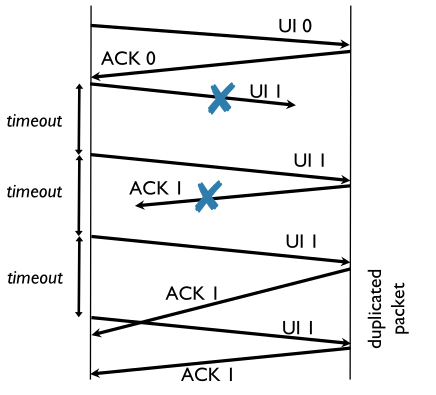
\includegraphics[width=0.4\columnwidth]{./images/esempio_comunicazione_stop_wait_no_sqn.png}
	\caption{Esempio comunicazione stop and wait senza SQN}
	\label{fig:esempio_comunicazione_stop_wait_no_sqn}
\end{figure}


\begin{figure}[!ht]
	\centering
	% TODO: ingrandire immagine a 0.4
	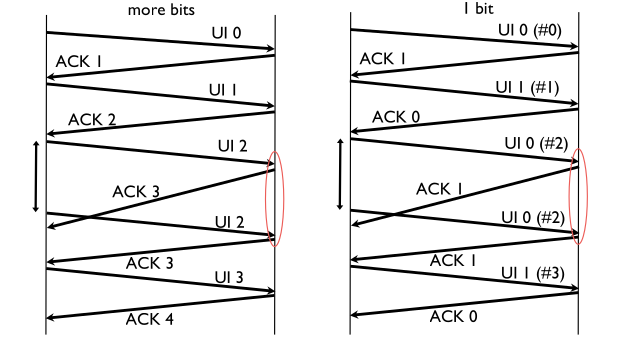
\includegraphics[width=0.4\columnwidth]{./images/esempio_comunicazione_stop_wait_sqn.png}
	\caption{Esempio comunicazione stop and wait con SQN}
	\label{fig:esempio_comunicazione_stop_wait_sqn}
\end{figure}



\subsubsection{Stop and wait performance}

I tempi considerati sono:
\begin{itemize}
	\item \textbf{$T_U$}: tempo di trasmissione di un pacchetto, misurato in $s/IU$
	\item \textbf{$T_P$}: tempo di propagazione di un pacchetto, misurato in $s/IU$
	\item \textbf{$T_{A}$}: tempo di trasmissione di un ACK, misurato in $s/IU$
\end{itemize}

Il tempo totale per inviare un'unità informativa(caso ideale):
\begin{align}
	T_{tot} = T_{U} + 2T_{P} + T_{A}
\end{align}

Il massimo grado di utilizzo di un canale di comunicazione nel caso di \textbf{assenza di errore}:
\begin{align}
	\rho_0
	 & =\frac{T_U}{T_{tot}}                                                     \\
	 & = \frac{T_U}{T_U + 2T_P + T_A}                                           \\
	 & = \begin{cases}
		     \frac{1}{2 + 2 \frac{T_P}{T_U}} \quad \text{se}\quad T_U = T_A  \\
		     \frac{1}{2 \frac{T_P}{T_U} + 1} \quad \text{se}\quad T_U >> T_A \\
		     0 \quad \text{se}\quad T_P >> T_U
	     \end{cases}
\end{align}



Nel caso di \textbf{presenza di errore}, non viene ricevuto l'ACK dal trasmettitore, devo fare alcune assunzioni:
\begin{itemize}
	\item Indipendenza statisticamente dei pacchetti informativi
	\item perdita di pacchetti ACK
\end{itemize}

Indico con $p$ la probabilità di perdita del pacchetto.


Il tempo per l'arrivo di un pacchetto con presenza di errori diventa:
\begin{align}
	\Bar{T_1} = & (N_t - 1) T_0 + T_1     \\
	=           & \frac{p}{1-p} T_0 + T_1 \\
	\simeq      & \frac{T_1}{1-p}
\end{align}

Dove $N_t$ è desscritta come:
\begin{align}
	N_t = \sum_{k=1}^{\infty} k p^{k-1} (1-p) = \frac{1}{1-p}
\end{align}

Quindi l'utilizzazione del canele diventa:
\begin{align}
	\rho = (1 - p) \rho_0
\end{align}


\subsubsection{Sliding window}
PAGINA 80
